\documentclass{beamer}
\usepackage{amsfonts}
\usepackage{amsmath}
\usepackage{amssymb}
\usepackage{amsmath}
\usepackage{algorithm}
\usepackage[noend]{algpseudocode}
\usepackage{amsthm}
\usepackage{mathtools}
\DeclarePairedDelimiter\abs{\lvert}{\rvert}

\begin{document}

\title{Primes and How to Recognize them}
\subtitle{Primality Testing Algorithms}
\author{Satwant Rana\inst{1}\\[3mm] Advised by, Amitabha Tripathi\inst{2}}
\institute
{
  \inst{1}
  2012 MT 50618\\
  Mathematics Department\\
  IIT Delhi
  \and
  \inst{2}
  Professor\\
  Mathematics Department\\
  IIT Delhi
}
\date
{MTP Presentation, 2016-17}
\subject{Mathematics}

\frame{\titlepage}

\begin{frame}
\frametitle{Motivation}

Prime numbers are central to Number Theory, acting as the atomic units around which all numbers are built. Therefore it is barely a surprise that \emph{Primality Testing} is a problem with a rich history in Number Theory.
\\[3mm]
The motivation behind this project is to rediscover, implement and understand some of the most important algorithms for primality testing.
\end{frame}

\begin{frame}
\frametitle{Primes and Composites}
Primes are defined as natural numbers which are only divisible by $1$ and themselves. Formally, given $p \in \mathbb{N}$ is a prime, if whenever $q \mid p$, then $q \in \{1, p\}$.
\\[3mm]
Any natural greater than $1$ which is not a prime is called a \emph{composite}.
\end{frame}

\begin{frame}
\frametitle{A Naive Primality Test}

\begin{algorithm}[H]
\caption{Naive Primality Test}
\label{alg:NaivePrimalityTest}
\begin{algorithmic}
\Procedure{NaivePrimalityTest}{$n$}
\State $d\gets 2$
\While {$d \leq n-1$}
\State $r \gets n \mod d$
\If {$r = 0$} 
	\State \textbf{return} false \Comment{$n$ is composite}
\EndIf
\State $d \gets d+1$
\EndWhile
\State \textbf{return} true \Comment{$n$ is prime}
\EndProcedure
\end{algorithmic}
\end{algorithm}
Time Complexity - $O(n)$

\end{frame}

\begin{frame}
\frametitle{An Optimization}

If $n,a,b \in \mathbb{Z}$ such that $n = ab$, then $min(a,b) \leq \sqrt n$.

\begin{algorithm}[H]
\caption{Optimized Naive Primality Test}
\label{alg:OptimizedNaivePrimalityTest}
\begin{algorithmic}
\Procedure{OptimizedNaivePrimalityTest}{$n$}
\State $d\gets 2$
\While {$d \leq \min(n-1,\sqrt n))$}
\State $r\gets n \mod d$
\If {$r = 0$} 
	\State \textbf{return} false \Comment{$n$ is composite}
\EndIf
\State $d \gets d+1$
\EndWhile
\State \textbf{return} true \Comment{$n$ is prime}
\EndProcedure
\end{algorithmic}
\end{algorithm}

Time Complexity - $O(\sqrt n)$
\end{frame}

\begin{frame}
\frametitle{Compositeness Tests}

A successful \emph{primality test} proves that a given number is prime, whereas a successful \emph{compositeness test} proves that a given number is composite. 
\\[3mm]
e.g. If $n > 2$ and $2 \mid n$, then $n$ is composite.
\\[3mm]
If a compositeness test is not successful, then we can't comment on the primality of the given number.
\\[3mm]
Composite numbers which the compositeness test labels as primes are called the \emph{pseudoprimes} for the test.

\end{frame}

\begin{frame}
\frametitle{Fermat's (Little) Theorem}

\begin{theorem}[Fermat's Theorem]
\label{theorem:FermatLittleTheorem}
Given prime $p$, and $a \in \mathbb{Z}$, $(a,p) = 1$ we have,
\[ a^{p-1} \equiv 1 \mod p \]
\end{theorem}

\begin{corollary}[1]
\label{corollary:BetterFermatLittleTheorem}
Given prime $p$, and $a \in \mathbb{Z}$ we have,
\[ a^p \equiv a \mod p \]
\end{corollary}

\end{frame}

\begin{frame}
\frametitle{Fermat's Theorem as a Compositeness Test}
The following Corollary 2 is a simple compositeness test using \emph{Fermat's Theorem}. 
\\[3mm]
\begin{corollary}[2]
\label{corollary:FermatLittleTheoremConverse}
If $n \in \mathbb{N}$, $n \geq 2$ and $\exists a \in \mathbb{Z}$ such that,
\[a^n \not\equiv a \mod n\]
then $n$ is not a prime.  
\end{corollary}
\ \\[3mm]
For instance, for $n = 9$, $2^9 \equiv 8 \not\equiv 2 \mod 9$, indicating the compositeness of $9$.

\end{frame}

\begin{frame}
\frametitle{Fermat Pseudoprimes}

There do exist combinations of $a$ and composite $n$ which satisfy the \emph{Fermat's Theorem}. 
\\[3mm]
For instance $n = 341 = 11.31$ gives $2^{341} \equiv 2 \mod 341$. This makes $341$ a pseudoprime to the Fermat's Compositeness Test, or a \emph{Fermat Pseudoprime}. 
\\[3mm]
Although, in this case a change of base $a$ from $2$ to $3$ yields $3^{341} \equiv 168 \not\equiv 3 \mod 341$ which indicates that $341$ is not a prime.

\end{frame}

\begin{frame}
\frametitle{Carmichael Numbers}

Given $n \in \mathbb{Z}$ is a \emph{Carmichael Number}, if $a^{n-1} \equiv 1 \mod n$, $\forall a \in \mathbb{Z}, (a,n) = 1$. 
\\[3mm]
The smallest example of \emph{Carmichael Numbers} is $561$, and there exist infinitely many of them.
\\[3mm]
\emph{Carmichael Numbers} are \emph{Fermat Pseudoprimes} for each base $a$ comprime to $n$.

\end{frame}

\begin{frame}
\frametitle{Eucledian Algorithm for G.C.D.}

For $a, b \in \mathbb{Z}$, we have $(a,0) = a$, $(a,b) = (a,b-a)$ and therefore $(a,b) = (a,b \mod a)$. 
\\[3mm]
\begin{algorithm}[H]
\caption{Euclidean Algorithm}
\label{alg:EuclideanAlgorithm}
\begin{algorithmic}
\Procedure{EuclideanAlgorithm}{$a, b$}
\State $a \gets \Call{Abs}{a}$
\State $b \gets \Call{Abs}{b}$ \Comment{Eliminating negative signs}
\If {$a > b$}
	\State \Call{Swap}{$a, b$} 
\EndIf
\While {$a \neq 0$}
	\State $c \gets b \mod a$
	\State $b \gets a$
	\State $a \gets c$
\EndWhile
\State \Return $b$
\EndProcedure
\end{algorithmic}
\end{algorithm}

Time Complexity - $O(\log \min(\abs a,\abs b))$
\end{frame}

\begin{frame}
\frametitle{Logarithmic Exponentiation}

\[a^n = \begin{cases} 
      1 & n = 0 \\
      (a^{\frac n 2})^2 & n \equiv 0 \mod 2 \\
      a(a^{\frac {n-1} 2})^2 & n \equiv 1 \mod 2 \\
   \end{cases}
\]

\begin{algorithm}[H]
\caption{Recursive Logarithmic Exponentiation}
\label{alg:RecursiveLogarithmicExponentiation}
\begin{algorithmic}
\Procedure{LogarithmicExponentiation}{$a, n, m$} 
\State $result \gets 1 \mod m$ \Comment{Calculates $a^n \mod m$}
\If {$n > 0$ \ \& \ $n \equiv 0 \mod 2$}
	\State $result \gets \Call{LogarithmicExponentiation}{a, \frac n 2, m}$
	\State $result \gets result * result \mod m$
\ElsIf {$n > 0$ \ \& \ $n \equiv 1 \mod 2$}
	\State $result \gets \Call{LogarithmicExponentiation}{a, \frac {n-1} 2, m}$
	\State $result \gets result * result \mod m$
	\State $result \gets result * a \mod m$
\EndIf
\State \Return $result$
\EndProcedure
\end{algorithmic}
\end{algorithm}

\end{frame}

\begin{frame}
\frametitle{Logarithmic Exponentiation}

If $n = b_{d-1}b_{d-2}\dots b_{0} = \sum_{i=0}^{d-1}b_i 2^i$, then
\[a^n = a^{\sum_{i=0}^{d-1}b_i 2^i} = \prod_{i=0}^{d-1} a^{b_i 2^i}\]

\begin{algorithm}[H]
\caption{Iterative Logarithmic Exponentiation}
\label{alg:IterativeLogarithmicExponentiation}
\begin{algorithmic}
\Procedure{LogarithmicExponentiation}{$a, n, m$}
\State $result \gets 1 \mod m$ \Comment{Calculates $a^n \mod m$}
\State $b \gets a$
\While {$n > 0$}
\If {$n \mod 2 = 1$} \Comment{If rightmost bit is 1 }
	\State $result \gets result * b \mod m$ \Comment{Multiply by $b$}
\EndIf
\State $b \gets b * b \mod m$ \Comment{$b$ stores $a^{2^i}$ on $i^{th}$ step}
\State $n \gets \frac n 2$ \Comment{Remove rightmost bit}
\EndWhile \label{euclidendwhile}
\State \Return result
\EndProcedure
\end{algorithmic}
\end{algorithm}
Time Complexity - $O(\log n)$
\end{frame}

\begin{frame}
\frametitle{Fermat's Compositeness Test}
Using current discussion, \emph{Fermat's Compositeness Test} can be implented as
\begin{algorithm}[H]
\caption{Fermat's Compositeness Test}
\label{alg:FermatCompositenessTest}
\begin{algorithmic}
\Procedure{FermatCompositenessTest}{$a, n$}
\State $gcd \gets \Call{EucledianAlgorithm}{a, n}$.
\If {$gcd > 1 \ \& \ gcd < n$}
	\State \Return $false$
\EndIf
\State $left \gets \Call{LogarithmicExponentiation}{a,n,n}$
\State $right \gets a \mod m$
\State \Return $left \neq right$
\EndProcedure
\end{algorithmic}
\end{algorithm}

\end{frame}

\begin{frame}
\frametitle{Fermat's Probabilistic Primality Test}

Every failed run of a compositness test reduces the probability of compositeness, and increases the probability of primality. So we have a \emph{Probabilistic Primality Test},

\begin{algorithm}[H]
\caption{Fermat's Probabilistic Primality Test}
\label{alg:FermatProbabilisticPrimalityTest}
\begin{algorithmic}
\Procedure{FermatProbabilisticPrimalityTest}{$n, iter$} 
\While {$iter > 0$} \Comment {$iter$ is number of iterations}
	\State $a \gets \Call{Random}{0,n-1}$ \Comment {Random number in $[0,n-1]$}
	\State $check \gets \Call{FermatCompositenessTest}{a,n}$
	\If {check}
		\State \Return $false$ \Comment {Composite found}
	\EndIf
	\State $iter \gets iter-1$
\EndWhile
\State \Return $true$ \Comment {Probable prime found}
\EndProcedure
\end{algorithmic}
\end{algorithm}

Time Complexity - $O(\log n)$

\end{frame}

\begin{frame}
\frametitle{Fermat's Primality Test}
If we have a table of \emph{pseudoprimes} then a simple check removes the flaw from \emph{Fermat's Compositeness Test}.
\\[3mm]
D.H. Lehmer prepared a table of all Fermat pseudoprimes below $2.10^8$ for the base $2$ with no factor $< 317$. Thus a primality test to check primality for $n < 2.10^8$ can be formulated.
\end{frame}

\begin{frame}
\frametitle{Fermat's Primality Test}
\begin{algorithm}[H]
\caption{Fermat's Primality Test}
\label{alg:FermatPrimalityTest}
\begin{algorithmic}
\Procedure{FermatPrimalityTest}{$n$} 
\If {$n \geq 2.10^8$}
	\State \Return $false$ \Comment {Fail if out of range}
\EndIf
\For {$i = 2$, $i \leq \min(313,n-1)$, $i \gets i+1$}
	\If {$i \mid n$}
		\State \Return $false$ \Comment {Factor $\leq 313$}
	\EndIf
\EndFor
\If {$\Call{IterativeLogarithmicExponentiation}{2,p-1,p} \not\equiv 1 \mod 2$}
	\State \Return $false$ \Comment {Composite by Fermat's Theorem}
\EndIf
\State \Return $!\Call{IsLehmerPseudoprime}{n}$ \Comment {Check Lehmer's Table}
\EndProcedure
\end{algorithmic}
\end{algorithm}

\end{frame}

\begin{frame}
\frametitle{A Generalization of Fermat's Theorem}
The reason why Fermat's Theorem can only be a used to create a Compositeness Test, is that it's only a necessary condition on primality. Here's a (generalized) necessary and sufficient generalization of Fermat's Little Theorem.
\\[3mm]
\begin{theorem}
\label{theorem:GeneralisedFermatLittleTheorem}
Given $n \in \mathbb{N}$, $n \geq 2$ and $a \in \mathbb{Z}$, $(a,n) = 1$, then $n$ is prime if and only if
\[ (X+a)^n \equiv X^n + a \mod n \]
\end{theorem}
\end{frame}

\begin{frame}
\frametitle{A Generalization of Fermat's Theorem}
A simple primality test - Choose an apt $a$, and then test the congruence $(X+a)^n \equiv X^n + a \mod n$. But there are $O(n)$ terms in the polynomial, making our test $\Omega(n)$.
\\[3mm]
One way to reduce the number of terms in the polynomial is to consider the congruences modulo $X^r-1$ additionally, for a small $r$.
\end{frame}

\begin{frame}
\frametitle{Build-up to a Polynomial Time Primality Test}
To make things concrete, we consider the congruence,
\[(X+a)^n \equiv X^n+a \mod (n, X^r-1)\]
and build a primality test around it.
\\[3mm]
The above congruence follows for prime $n$ as before, but depending upon how small $r$ we chose, some composite values of $n$ may also satisfy the congruence now.
\\[3mm]
\emph{AKS Primality Test} uses a polynomial $r$, and a polynomial number of values of $a$ to deduce whether $n$ is a prime or not. 
\end{frame}

\begin{frame}
\frametitle{AKS Primality Test}
\begin{algorithm}[H]
\caption{AKS Primality Test}
\label{alg:AKSPrimalityTest}
\begin{algorithmic}
\Procedure{AKSPrimalityTest}{$n$} 

\If {$n < 2$ or $n = a^b$ for $a, b \in \mathbb{N}$ and $b \geq 2$}
	\State \Return $false$  \Comment {Step 1}
\EndIf

\State $r \gets min \{i: i \in \mathbb{N},\ i \leq \max(3,\ \lceil \log^5 n \rceil),\ o_i(n) > \log^2 n \}$ \Comment {Step 2}

\For {$a = 2$, $i \leq r$, $a \gets a+1$}
	\If {$1 < (a,n) < n$}
		\State \Return $false$  \Comment {Step 3}
	\EndIf
\EndFor

\If {$n \leq r$}
	\Return $true$  \Comment {Step 4}
\EndIf

\For {$a = 1$, $a \leq \lfloor \sqrt{\phi(r)} \log n \rfloor$, $a \gets a+1$}
	\If {$(X+a)^n \not \equiv X^n + a \mod (n, X^r - 1)$}
		\State \Return $false$  \Comment {Step 5}
	\EndIf
\EndFor
\State \Return $true$ \Comment {Step 6}
\EndProcedure
\end{algorithmic}
\end{algorithm}
Time complexity - $\tilde O(r^\frac{3}{2}log^3 n) = \tilde O(log^{10.5} n)$
\end{frame}

\begin{frame}
\frametitle{AKS Primality Test - Prime Input}
\begin{lemma}
\label{lemma:AKSLemma1}
If $n$ is a prime then Algorithm~\ref{alg:AKSPrimalityTest} returns $true$.
\end{lemma}
\begin{proof}
If $n$ is a prime, then Steps $1$ and $3$ can never return $false$. Also by previous discussion, Step $5$ can't return $false$. So the algorithm returns $true$ in either Step $4$ or Step $6$.
\end{proof}
\end{frame}

\begin{frame}
\frametitle{AKS Primality Test - Is $n$ a perfect power?}
\begin{algorithm}[H]
\caption{Perfect Power Test}
\label{alg:PerfectPowerTest}
\begin{algorithmic}
\Procedure{PerfectPowerTest}{$n$}
\If {$n = 1$}
	\State \Return $true$
\EndIf
\For {$b \gets 2$, $b \leq \log n, b \gets b+1$}
	\State $l \gets 1, u \gets n$
	\While {$l < u$}
		\State $m \gets \lfloor \frac{l+u}{2} \rfloor$
		\State $x \gets m^b$ \Comment{Use Logarithmic Exponentiation here}
		\If {$x = n$}
			\ \Return $true$
		\ElsIf {$x < n$}
			\ $l \gets m+1$
		\Else
			\ $r \gets m-1$
		\EndIf
	\EndWhile
\EndFor
\State \Return $false$
\EndProcedure
\end{algorithmic}
\end{algorithm}
Time Complexity - $O(\log^4 n)$
\end{frame}

\begin{frame}
\frametitle{AKS Primality Test - Existence of a small $r$}

\begin{lemma}
\label{lemma:LCMLemma}
Let $LCM(m)$ be $lcm$ of first $m$ numbers. We have for $m \geq 7$,
\[LCM(m) \geq 2^m\]
\end{lemma}

\begin{lemma}
\label{lemma:AKSLemma2}
There exists an $r \leq \max(3, \lceil \log^5 n \rceil)$ and $o_r(n) > \log^2 n$.
\end{lemma}
\ 
\\[3mm]
Consider the smallest $r \in \mathbb{N}$ which doesn't divide the product $P$ defined as,
\[P = n^{\log B}\ .\ \prod_{i=1}^{\lfloor \log^2 n \rfloor}{n^i-1} \]

\end{frame}

\begin{frame}
\frametitle{AKS Primality Test - Some definitions}
Remaining case is of composite $n$. Let $p | n$, such that $o_r(p) > 1$. So $(p,r) = (n,r) = 1$.
\[\forall\ 0 \leq a \leq l\]
\[(X+a)^n \equiv X^n + a \mod (n, X^r - 1)\]
\[(X+a)^p \equiv X^p + a \mod (p,X^r-1)\]
\[\implies ((X+a)^p)^{\frac{n}{p}} \equiv (X^p)^{\frac{n}{p}} + a \mod (p, X^r - 1)\]
\[\implies (X^p+a)^{\frac{n}{p}} \equiv (X^p)^{\frac{n}{p}} + a \mod (p, X^r - 1)\]
\[\implies (X+a)^{\frac{n}{p}} \equiv X^{\frac{n}{p}} + a \mod (p, X^r - 1)\]
\end{frame}

\begin{frame}
\frametitle{AKS Primality Test - Some definitions}
\begin{definition}
\label{definition:introspective}
For polynomial $f(X)$ and $m \in \mathbb{N}$, if $m$ satisfies
\[f(X)^m \equiv f(X^m) \mod (p,X^r-1)\]
then $m$ is said to be introspective for $f(X)$.
\end{definition}

\begin{lemma}
\label{lemma:IntrospectiveLemma1}
If $m$ and $m'$ are both introspective for a polynomial $f(X)$, then so is $m . m'$.
\end{lemma}

\begin{lemma}
\label{lemma:IntrospectiveLemma2}
If $m$ is introspective for both the polynomials $f(X)$ and $g(X)$, then it is also introspective for $f(X) . g(X)$.
\end{lemma}
\end{frame}

\begin{frame}
\frametitle{AKS Primality Test - About two groups}
Every number in the set $I = \{\frac{n}{p}^i.p^j\ |\ i,j \in \mathbb{N}_0\}$ is introspective for every polynomial in the set $P = \{\prod_{a=0}^{l}{(X+a)^{e_a}}\ |\ e_a \in \mathbb{N}_0\}$.
\\[3mm]
The first group is the set of residues of all elements of $I$ modulo $r$. Let's denote this set as $G$, and it is a subset of $\mathbb{Z}_r^*$ as $(n,r) = (p,r) = 1$. Let $t = |G|$. Since $n^i \in G \ \forall \ i \in \mathbb{N}_0$ and $o_r(n) > \log^2(n)$, we have $t > \log^2(n)$.
\\[3mm]
Let $Q_r(X)$ be $r^{th}$ cyclotomic polynomial over $F_p$. $Q_r(X)$ divides $X^r-1$ and factors into irreducible factors of degree $o_r(p)$. Let $h(X)$ be one such irreducible factor. Since $o_r(p) > 1$, degree of $h(X)$ is greater than one. The second group is the set of all residues of polynomials in $P$ modulo $h(X)$ and $p$. Let $\mathcal{G}$ be this group. This group is generated by elements $X, X + 1, X + 2, \dots, X + l$ in the field $F = F_p[X]/(h(X))$ and is a subgroup of the multiplicative group of $F$.
\end{frame}

\begin{frame}
\frametitle{AKS Primality Test - Estimating the size of $\mathcal{G}$}
\begin{lemma}
[Lenstra]\label{lemma:GLowerBound}
$|\mathcal{G}| \geq {{t+l} \choose {t-1}}$
\end{lemma}
\ 
\\[3mm]
\begin{lemma}
\label{lemma:GUpperBound}
If $n$ is not a power of $p$, then $|\mathcal{G}| \leq n^{\sqrt{t}}$
\end{lemma}
\end{frame}

\begin{frame}
\frametitle{AKS Primality Test - Completing the proof}
\begin{theorem}
If Algorithm~\ref{alg:AKSPrimalityTest} returns $true$ then input $n$ is prime.
\end{theorem}
\[|\mathcal{G}| \geq {{t+l} \choose {t-1}}\]
\[|\mathcal{G}| \geq {{{\lfloor \sqrt t \log n \rfloor} + 1 + l} \choose {\lfloor \sqrt t \log n \rfloor}}\]
\[|\mathcal{G}| \geq {{2{\lfloor \sqrt t \log n \rfloor}+1} \choose {\lfloor \sqrt t \log n \rfloor}}\]
\[|\mathcal{G}| \geq 2^{{\lfloor \sqrt t \log n \rfloor}+1} > 2^{\sqrt t \log n} = n^{\sqrt t}\]
So $n$ is a power of $p$, which contradicts the structure of Algorithm~\ref{alg:AKSPrimalityTest}.

\end{frame}

\begin{frame}
\frametitle{Implementation and Simulations}
\begin{figure}
 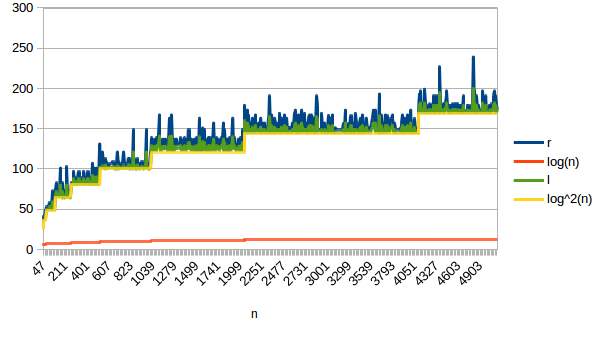
\includegraphics[width=\linewidth / 2]{../data/aks/n-r-l-5000.png}
 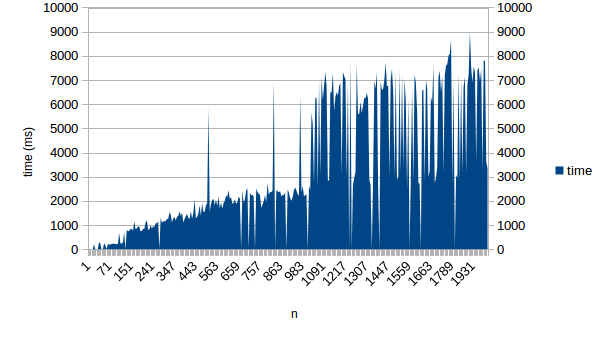
\includegraphics[width=\linewidth / 2]{../data/aks/n-time-2000.png}
 \caption{AKS simulations for various values of input $n$.}
\end{figure}
Implementation exists at \\\texttt{https://github.com/satwantrana/primality-testing}.
\end{frame}

\begin{frame}
\frametitle{A generalisation of AKS}
\begin{theorem}
\label{theorem:GeneralizedAKS}
Given $n, r \in \mathbb{N}$ and $S \subseteq \mathbb{N}$ such that,
\begin{enumerate}[1.]
\item $n$ can be written as a product of elements from $S$.
\item $S$ is not generated, under multiplication, by a proper subset of $S$.
\item $(n, r) = 1$ and $o_r(n) > \log^{1 + \frac 1 {k}} n$.
\item $(X+a)^m \equiv X^m + a \mod (X^r-1, n)\ \forall \ m \in S$ and $1 \leq a \leq l_k$.
\end{enumerate}
where $k = |S|$, $\displaystyle N = \prod_{m \in S} m$ and $l_k = \lfloor \phi(r)2^{log_n N}\rfloor$; then $n$ is power of a prime. 

Further, such an $r$ exists which is prime with $r \leq \log^{3 + \frac{2}{k}} n$. Also, if $o_r(N) > log^{1 + \frac{1}{k}} N$, then $l_k$ gets improved to $\lfloor \phi(r)^\frac{1}{k+1} log N \rfloor$ with such an existing with $r \leq \log^{3 + \frac{2}{k}} N$.
\end{theorem}
Time complexity - $\tilde O(l_k \cdot \log N \cdot r \cdot \log n)$
\end{frame}

\begin{frame}
\frametitle{More introspective numbers}
\begin{lemma}
\label{lemma:MoreIntrospectiveNumbers}
Given distinct primes $n$, $r \in \mathbb{N}$, then $\forall f(X) \in \mathbb{Z}[X]$,
\[f(X)^{n^{\phi(r)}-1} \equiv 1 \mod (n, X^r - 1)\]
\end{lemma}

\begin{corollary}
\label{corollary:MoreIntrospectiveNumbersCorollary}
If $n$ and $r$ are primes, then $\{n + \lambda (n^{\phi(r)} - 1): (\lambda, n) = 1 \}$ is an infinite set of introspective numbers, all of which are coprime to $n$, for all polynomials $f(X) \in \mathbb{Z}[X]$.
\end{corollary}
\end{frame}

\begin{frame}
\frametitle{Conclusion}
\center{... and Thank You!}
\end{frame}
\end{document}